\documentclass{cmspaper}
\usepackage{graphicx}
\usepackage{amssymb}
\usepackage{amsmath}
%\usepackage{draft}
\usepackage{lineno}
\usepackage[table]{xcolor}
\usepackage{url}

\linenumbers % For draft version

%----------------------------------------
% On ins�re ici les diff�rentes parties du rapport 
%----------------------------------------

\begin{document}

\begin{titlepage}
\internalnote{IN-2013/XXX}
%\cmsnote{2007/000}
\date{\today}
\title{System Architecture for CMS L1 Tracking Trigger and work plan for Vertical Slice System Demonstration}
\begin{Authlist}
%G.~Baulieu~\Aref{a}, C.~Combaret~\Aref{a}, R.~Dell~Orso~\Aref{b}, T.~Liu~\Aref{c}, L.~Martini~\Aref{b}, L.~Mirabito~\Aref{a}, F.~Palla~\Aref{b}, S.~Viret~\Aref{a}
\end{Authlist}

%\Anotfoot{a}{Institut de Physique Nucl\'eaire, UCBL, CNRS-IN2P3, Lyon, France}
%\Anotfoot{b}{INFN, Pisa, Italy}
%\Anotfoot{c}{Fermilab, USA}

\begin{abstract}
In this document we will describe a track trigger architecture and system demonstration as a proposal for Phase 2 tracking trigger R\&D for CMS. This will be a living document, serving multiple purposes. It is intended to define the tracking trigger project and organize the efforts towards the Technical Proposal, the Vertical Slice Demonstration System, and the TDR (Technical Design Report). It will be written in such a way to make it easy not only for new groups to learn, but also to communicate with all the relevant tracker, trigger and physics groups.
\end{abstract}
\end{titlepage}
\newpage
\tableofcontents
\newpage

%
% Uncomment the part you are interested in 
%

\begin{center}
{\Large\bf Executive summary}
\end{center}

\vspace{0.5cm}

\noindent A powerful tracking trigger is required for the success of the CMS physics program in the HL-LHC era.  Consequently, the design of the Phase-II CMS Tracker must allow for an effective implementation of the tracking trigger.  Although the construction of the Phase-II Tracker will take many years, the system's design must be finalized soon.  A silicon-based L1 tracking trigger has never been realized at this scale and thus it is imperative that the feasibility of the trigger be demonstrated before the design of the Phase-II Tracker is finalized.  A silicon-based track trigger was successfully used as part of the L2 CDF trigger (SVT) and is presently being implemented at L2 in ATLAS (FTK).  Both implementations employed an associative memory (AM) approach.  The experiences of these projects will serve as useful inputs in the design of the CMS L1 tracking trigger, however the higher occupancies anticipated in HL-LHC operation and the low latencies required at L1 present us with a unique set of challenges.

\noindent Motivated by these challenges, CMS has carried out a focused R\&D program to advance the state-of-the-art in hardware-based pattern recognition and track reconstruction.  We have attempted to address the issues of occupancy and latency by developing a ``full-mesh'' ATCA data formatting system, higher density AM chips and new algorithms for hardware-based track finding.  The long-term goal of this R\&D effort is to develop these critical technologies to the point where we can ultimately propose them as a viable solution to the problems of HL-LHC L1 track triggering.  Given the progress made by the R\&D program in the last few years, we believe it is now time to take the important next step of establishing a Vertical Slice Demonstration System.  This system will comprise a full tracking trigger path and will be used with simulated high-luminosity data to measure trigger latency and efficiency, to study overall system performance, and to identify potential bottlenecks and appropriate solutions.

\noindent The full-mesh ATCA architecture we have proposed for the CMS L1 tracking trigger permits high bandwidth inter-board communication.  The full-mesh backplane is used to time-multiplex the high volume of incoming data (~50Tbps) in such a way that I/O demands are manageable at the board and chip level.  The resulting architecture is scalable, flexible, and open and it enables us to undertake an early technical demonstration using existing technology.  The ATCA architecture will allow us to explore and compare various pattern recognition architectures and algorithms within the same platform.  Given that Advanced Mezzanine Card (AMC) specifications are designed to work with both ATCA and microTCA, the architecture naturally allows for the long-term integration of Tracker DAQ (AMC based) and tracking trigger activities.  

\noindent The proposed architecture and system demonstration has been well received in the Phase-II Tracker Upgrade community and we are now working to better define the concepts.  In this document we will describe the tracking trigger architecture and system demonstration as a work plan we propose for CMS Phase-II R\&D.  This {\itshape living document} is intended to define the tracking trigger project and to organize efforts leading to the Technical Proposal, the Vertical Slice Demonstration System and the Technical Design Report.



\clearpage

\section{Introduction}

\noindent Level-1 trigger (L1) is the first stage of CMS triggering system. This is a purely hardware stage during which LHC data rate is currently reduced from 20MHz to 100kHz within a latency of $6.4~\mu s$. Because of this very short latency, only the calorimeters and the muon subdetectors are part of L1 for the moment. The tracking detectors are used only at the second stage, knwon as the High-Level Trigger (HLT). 

\noindent Fig.~\ref{fig:L1Rates} illustrates how the lack of tracking at L1 might affect trigger efficiency. This figure shows, at LHC nominal luminosity, the rates of muons as a function of $p_T$. The line shows the generated muon rate, while black stars and red dots show muon rates after HLT and L1 respectively. The L1 muon rate, obtained using only the muon spectrometer, is much higher than the generated rate. It means that a lot of fake muons pass this trigger. These fakes are then cleaned at the HLT, as tracker info provides a much better sensitivity to muon identification than coarse muon info.
 
\begin{figure}[ht!]
\begin{minipage}[t]{7.5cm}
\centering
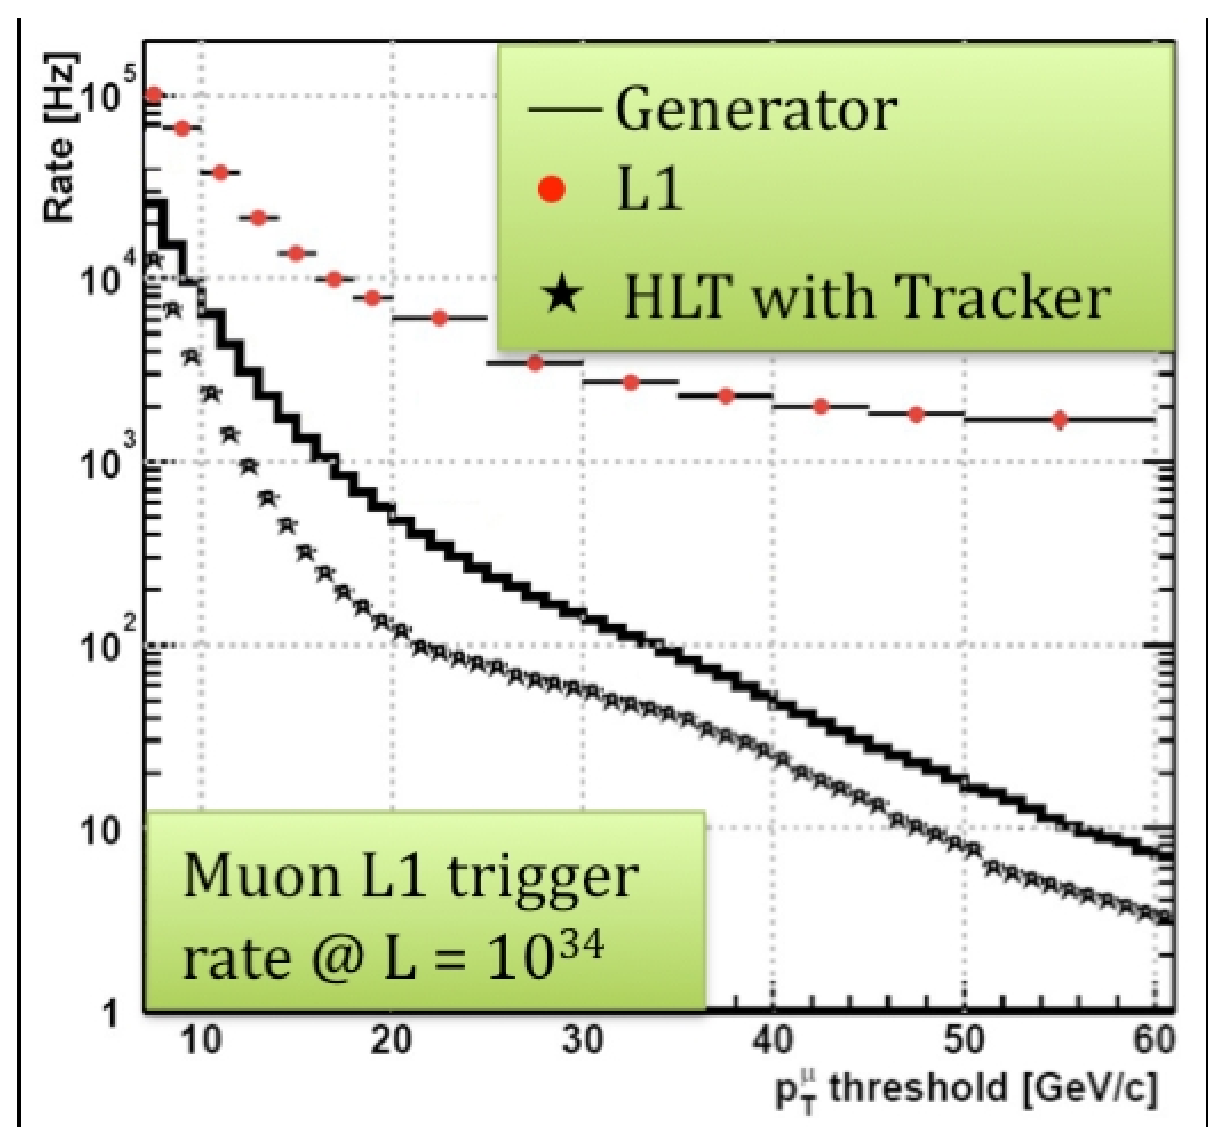
\includegraphics[width=0.99\textwidth]{Plots/CurrentTracker.eps}
\caption{Expected Level-1 single muon rate as a function of $p_{T}$ threshold for a luminosity of $10^{34}cm^{-2}s^{-1}$, in the present system.~\cite{bib:Abb-11}}
\label{fig:L1Rates}
\end{minipage}
\hfill
\begin{minipage}[t]{7.5cm}
\centering
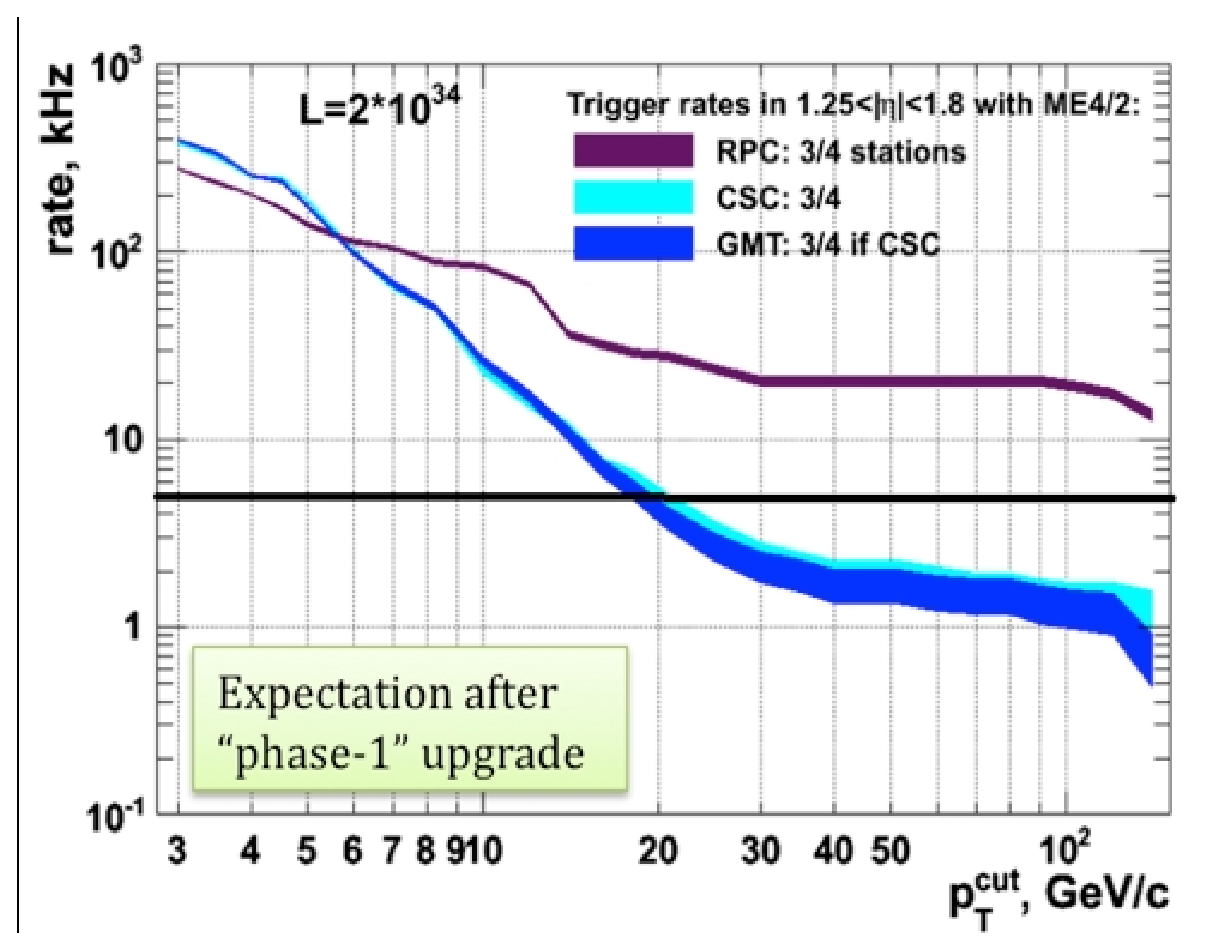
\includegraphics[width=0.99\textwidth]{Plots/21034_tracker.eps}
\caption{Expected threshold after phase 1 trigger upgrade, for a luminosity of $2\times 10^{34}cm^{-2}s^{-1}$.~\cite{bib:Abb-11}}
\label{fig:L1RatesPhase1}
\end{minipage}
\end{figure} 

\noindent One can also see on Fig.~\ref{fig:L1Rates} that fake proportion increases w.r.t. the $p_T$. This is due to the fact that L1 muon system uses coarse resolution information. Therefore high-$p_T$ tracks becomes compatible with straight lines at a certain point, and consequently the L1 muon rate reaches a plateau at high-$p_T$. At $10^{34}cm^{-2}s^{-1}$, this plateau lies at around $1~kHz$. Considering that overall L1 rate is $100~kHz$, the poor discrimination power at high-$p_T$ is not critical.

\noindent However, the plateau level is strongly depending on the instantaneous luminosity. Fig.~\ref{fig:L1RatesPhase1} shows its evolution, for the different muon subdetectors, at $2\times 10^{34}cm^{-2}s^{-1}$. For the RPC, the plateau lies at $20~kHz$, 20\% of the total L1 bandwidth. This is clearly not sustainable anymore. When going to HL-LHC luminosity, the other muons subdetectors also become problematic. In other words, muon indentification is not possible anymore. From there two solutions can be envisaged: increasing the L1 rate or including the tracking at L1. This note is dedicated to the second point.  

\noindent Our aim, in this document, is to procide a detailed description of such a system in the context of CMS. We tried to emulate the different stages of the hardware track fitting in order to estimate the feasibility/scaling of such a system with tracker geometry foreseen for CMS phase II upgrade. The simulation context, along with some estimation of the data rates that will be send to the trigger boards are presented in Section~{sec:FWork}. Pattern recognition is then described in Section~{sec:AM}. Finally, fitting stage is explained in Section~{sec:Fit}.

\clearpage

\section{CMS Track Trigger System Overview}

\subsection{Overview}

\noindent Extracting track information is a two-stage process. First of all, you have to retrieve the hits belonging to the track: this is the pattern recognition. Then, you extract the track parameters (momentum, impact parameter,...) from the hits: this is the fit. Both steps are performed routinely in CMS, using very performant software algorithms. In order to pass to L1, tracking has to go hardware.

\begin{figure}[ht!]
\centering
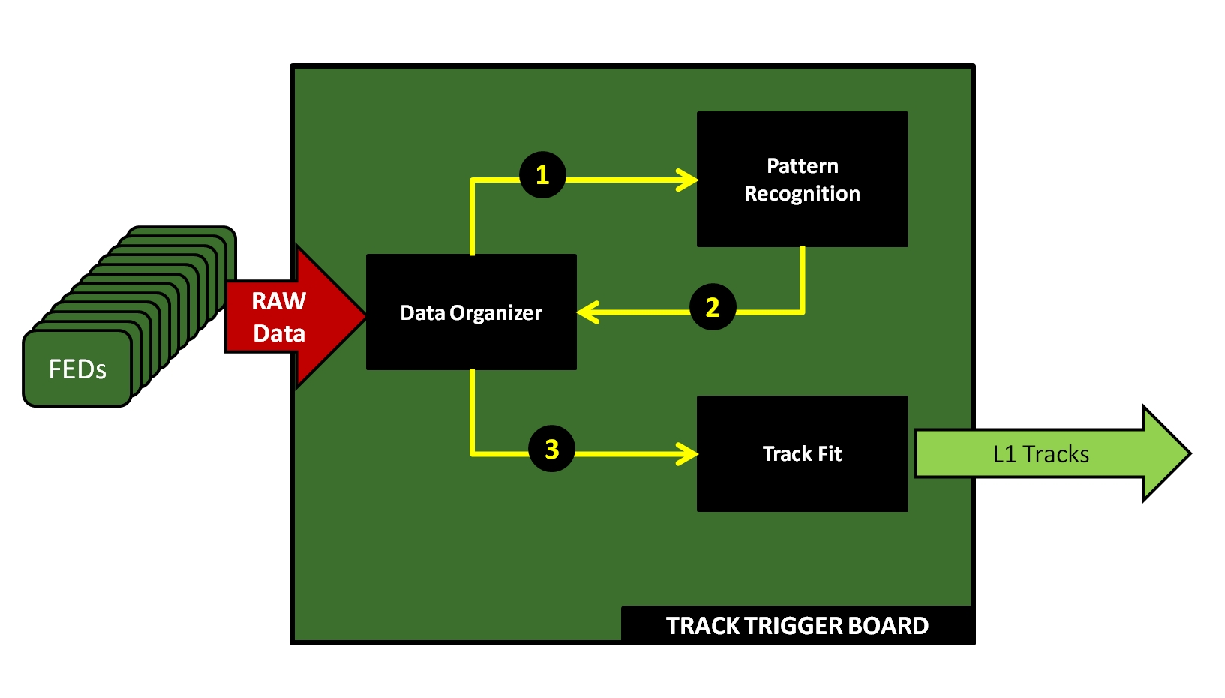
\includegraphics[width=0.5\columnwidth]{Plots/L1TTrigPrinciple.eps}
\caption{Hardware tracking principle}
\label{fig:L1TT_principle}
\end{figure}

\noindent Hardware-based tracking triggers were already developped in HEP experiments, in particular in the CDF experiment at Fermilab. Based on this system, the ATLAS experiment is planning to use a tracking trigger at the HLT after LHC long shutdown 2 in 2016. The working principle of these systems is sketched on Fig.~\ref{fig:L1TT_principle}. Tracker data is extracted by the FEDs and transmitted to the trigger board. Then, the data is handled by a data organization unit (DO), which extract the info necessary to the pattern recognition (PR), send it to the PR unit, and retrieve the matched patterns. The DO then sent the interesting hits to the track fit unit (TF), when the track parameters are estimated and sent to the L1 central trigger board.

\noindent In order to go at L1, one thus need the three following points: 

\begin{itemize}
\item A fast front-end readout system able to extract quickly all the data contained in the tracking detectors.
\item A system performing a fast pattern recognition.
\item A system performing a fast track fit.
\end{itemize}

\subsection{Interfaces}

\subsection{System architecture}

The associative memory system performs pattern recognition by comparing hits (stubs) with a reduced resolution with a large number
of prestored patterns almost in real time. 

The system is composed of mainly three parts: a data formatter (DF), which prepares the data at the reduced granularity to be transferred 
to the Associative Memory chip (AMchip), where the comparison with the patterns is performed and a list of matched patterns
is returned back. The hits at full granularity are then retrieved from the DF for the final track fitting stage (TF).

The reduced granularity compromises between the need to reduce to a manageable number of patterns to be stored in the AMchips, 
and the task of reducing the number of combinatorics in the Track Fitter stage. The AMchip stage thus overcomes the difficulties
of an approach based entirely on a fast processors architecture.

We will discuss the different tasks and their impact on the latency of the overall system. We will further address
a possible "state of the art" approach and what are the relevant directions of R\&D towards the final approach.


\subsubsection{The Data organizer}

\subsubsection{The AM chip}

The AMchip is based on an array of CAM cells. Columns of vertical buses distribute (bitlines) the hit information from each 
tracker layer to rows which contain the patterns. The rows perform writing of the patterns in the cell memory and matching 
functions. In the current AM06chip design, each bitline bus is composed of 18 bits in a hit and 18 corresponding inverted bits.
Every row is organized in sub-blocks of 8 CAMs cells (layer block), which is suited for the needs of FTK. Eventually these
will become equal to the number of needed layers of the CMS tracker. A pattern is a collection of 8 layer blocks, thus allowing
the identification of tracks crossing up to 8 layers. A logic is implemented to allow pattern matching with a pre-defined 
number of minimum blocks (8 or at least 7, for instance). The hit positions are received over 8 input buses of 15 bits each,
thus allowing a maximum of approximately 32K positions per each layer. The choice of 15 bits is taylored to the needs of FTK,
and could possibly be optimized for CMS. Actually of the 18 CAM cells each storing one bit, FTK uses 12 to store the 
12 most significant bits of the word, and 6 are used in 3 pairs and used a ternary cells, allowing for 0, 1 or X values, the 
X value meaning "don't care", so that the hits present on the hit bus will match the stored word regardless of the values
of the bits set to X. 


\subsection{Technical demonstrator concept}


\clearpage

\section{Pattern recognition and track fitting approaches}

\subsection{Introduction to associative memory approach}

\noindent Using associative memories in order to perform a fast pattern recognition (PR) at the trigger stage was first exposed in Ref.~\cite{bib:Del-89}. The principle is sketched in Fig.~\cite{fig:AM_principle}:
\begin{figure}[ht!]
\centering
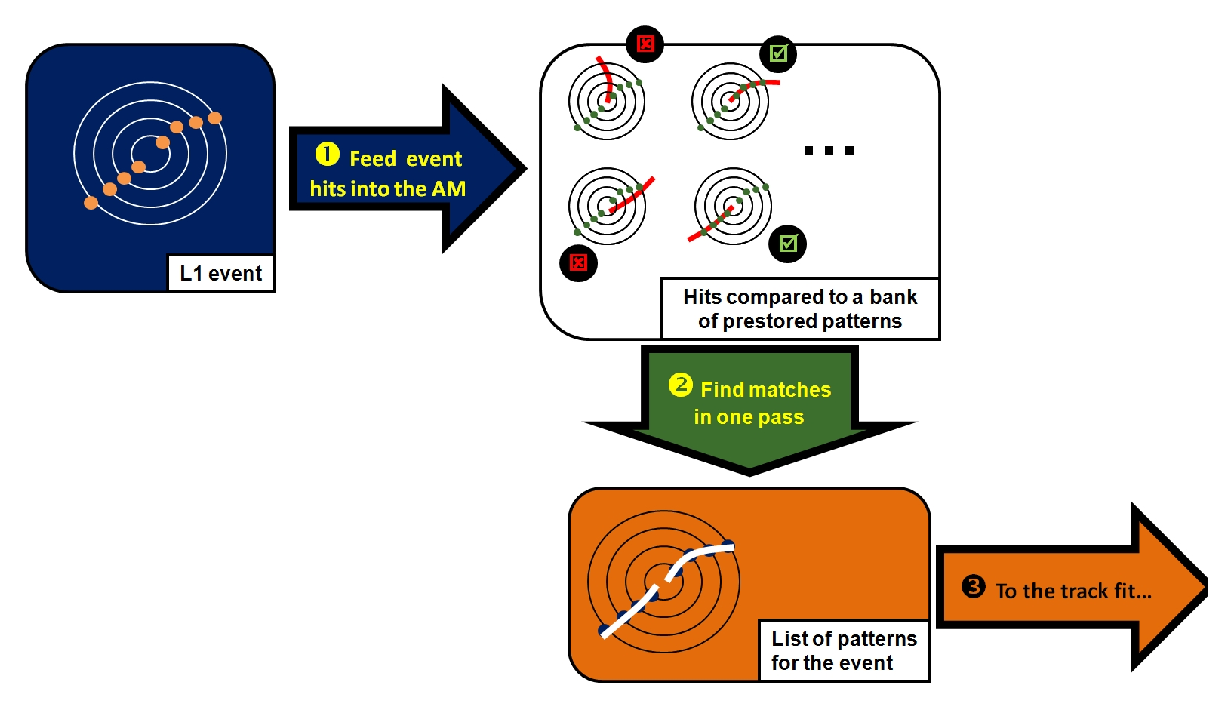
\includegraphics[width=0.7\columnwidth]{Plots/TriggerAM.eps}
\caption{Pattern recognition using associative memories.}
\label{fig:AM_principle}
\end{figure}

\noindent The idea is to compare the hits recorded in the tracking system to a bank of patterns stored in an associative memory chip. The patterns could be seen as low-granularity tracks, they are defined once for all using Monte-Carlo events, and they are ideally covering all the possible tracks occuring in the detector. In this part we will concentrate ourselves on the pattern bank definition. This is indeed the central point of the PR stage. The bank, which is defined using simulated events, has to fulfill few requirements. Before presenting them, it's important to define some parameters. 

\subsection{System configuration}

\subsubsection{Dividing the tracking system into sectors}

\noindent Before defining more precisely the pattern itself, one could introduce a very simple way to reduce the bank size, based on cyclindrical symmetry of the system. Tracker barrels and endcaps could indeed be azimuthally divided into symmetric sectors. The first stage to reduce the bank size will therefore be to generate banks for sectors, not for the whole detector. This doesn't mean that the banks will be exactly identical for all sectors, however, this will reduce the size of the banks to store.

\noindent It is tempting, at this stage, to divide the detector into very small sectors, in order to work with smaller banks. However, the minimal sector size is geometrically constrained by the track trigger requirements. The system should indeed be able to detect tracks over a given $p_T$ threshold (in our case $2~GeV/c$). The minimal sector should thus entirely contain such tracks. The maximum angular deviation of the particles we are looking for is easy to compute.
\begin{figure}[ht!]
\centering
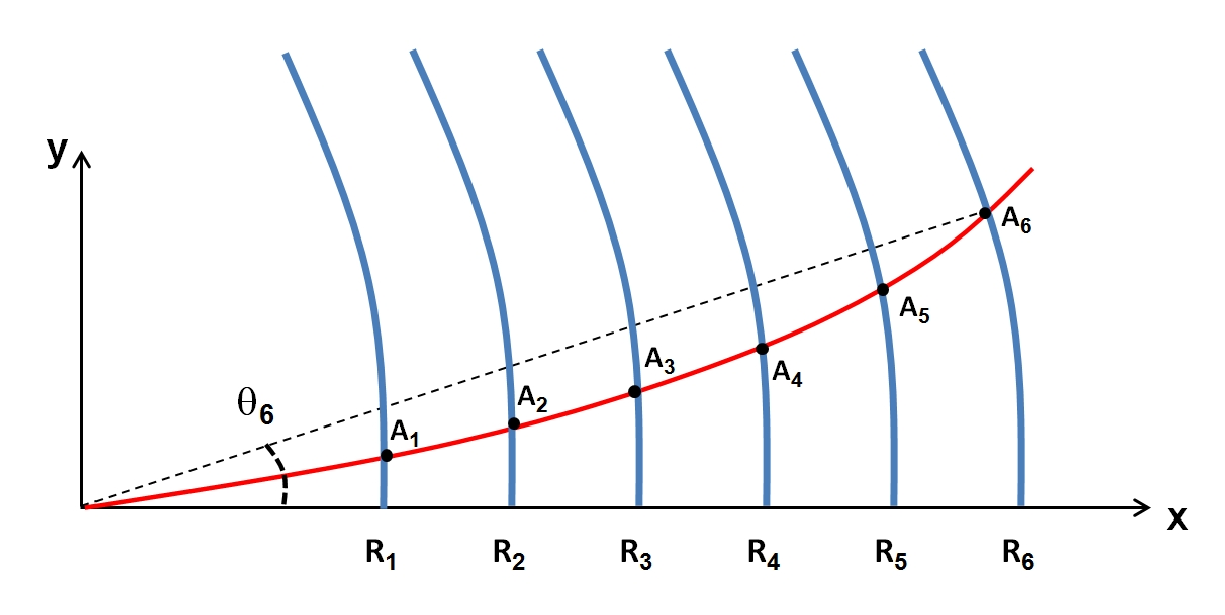
\includegraphics[width=0.6\columnwidth]{Plots/Deviations.eps}
\caption{Particle deviation in the different layers.}
\label{fig:Deviat}
\end{figure}

\noindent Using the notations of Fig.~\ref{fig:Deviat}, and considering that the particle has a curvature $R_c$, and is tangent to the x-axis at origin, one easily gets the coordinates $(x_i,y_i)$ of the points $A_i$, where the particle is crossing the layers (see Sec.~\label{sec:STUB}). The angular deviation is then given by:
\begin{equation}
\theta_i = atan \frac{y_i}{x_i} = atan \left(\frac{R_i}{2R_c}(1+\frac{R_i^2}{8R_c^2})\right)
\end{equation}  

\noindent For a particle with  $p_{T} = 2~GeV/c$ in a magnetic field $B_0 = 3.8~T$, the curvature radius is $R_c = 1.75~m$. From there, using the barrel-endcap geometry barrel layers radii, one can easily deduce the corresponding angular deviations. Values are summarized in Table~\ref{tab:dev}

\begin{table}[ht!]
\centering
\begin{tabular}{r|cccccc}
  \hline\hline
  Layer & 1 & 2 & 3 & 4 & 5 & 6\\
  \hline
  Radius (in m) & 0.23 & 0.384 & 0.524 & 0.699 & 0.874 & 1.08 \\
	\hline
  Deviation (in �) & 3.8 & 6.3 & 8.6 & 11.5 & 14.4 & 17.9 \\
  \hline\hline
\end{tabular}
\caption{The angular deviation of a primary particle with the minimal $p_T$ of $2~GeV/c$.}
\label{tab:dev}
\end{table}

\noindent From this result one can conclude that 36� in $r/\phi$ are sufficient to contain the trajectory of all charged particles with a $p_T$ larger than $2~GeV/c$ . We could thus divide the tracker area into overlapping sectors (e.g. 16 sectors of 45�), as shown on Fig.~\ref{fig:SEC_PHI}, and define one pattern bank per sector (which should be the same if the sectors are perfectly symetric in $r/\phi$) instead of a bank for the whole detector. 

\begin{figure}[ht!]
\begin{minipage}[t]{7.5cm}
\centering
\includegraphics[width=0.75\textwidth]{Plots/GeomSec.eps}
\caption{Overlap between sectors using a geometric definition}
\label{fig:SEC_PHI}
\end{minipage}
\hfill
\begin{minipage}[t]{7.5cm}
\centering
\includegraphics[width=0.75\textwidth]{Plots/AdapSec.eps}
\caption{Overlap between sectors using a module based definition}
\label{fig:SEC_MOD}
\end{minipage}
\end{figure} 

\noindent In practice, precise sector definition is slightly more complicated. Indeed one has to take into account modules granularity. A strict sector definition would be based on angular consideration only, and consequently contain only fraction of modules. Sticking to that definition would imply the ability to readout only some fraction of the modules. This is technically possible (a chip is 1/8th of a module), but would quickly become cumbersome to setup correctly. We have to keep in mind that the data will have to be sent to different trigger boards at very high rates, and cannot afford a complex cabling. The sector definition will therefore look like the one shown on Fig.~\ref{fig:SEC_MOD}.

\noindent For $\eta$, the situation is a bit more simpler as segmentation is thicker. In this study, we decided to divide each detector side into three $\eta$ regions:
\begin{itemize}
\item {\bf Barrel only:} for tracks with $0<\eta<0.9$.
\item {\bf Barrel+Endcap:} for tracks with $0.85<\eta<1.4$.
\item {\bf Endcap only:} for tracks with $1.35<\eta<2.2$. 
\end{itemize}  

\noindent For the $\phi$ part of the problem, the sectors were defined using two Monte Carlo samples of particle gun $\mu^{\pm}$ with a $p_T$ of $2~GeV/c$. The procedure is sketched in Fig~\ref{fig:sector_def}, and is the following:
\begin{figure}[ht!]
\centering
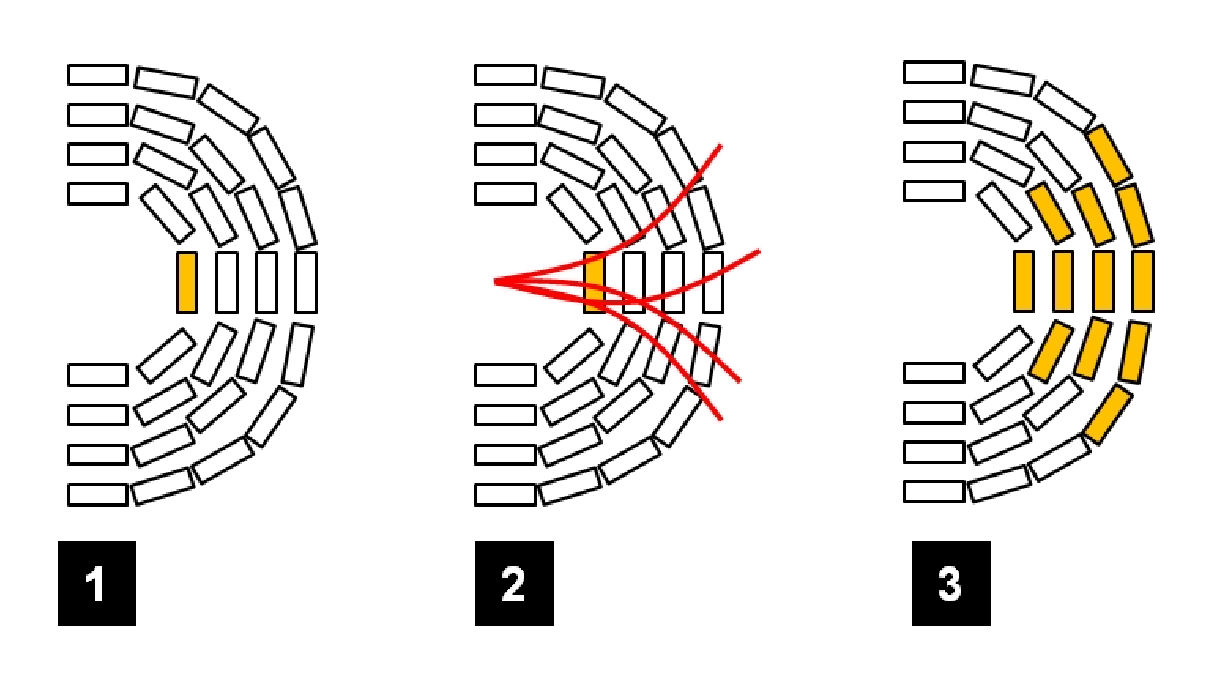
\includegraphics[width=0.6\columnwidth]{Plots/SectorDefinition.eps}
\caption{The sector definition procedure.}
\label{fig:sector_def}
\end{figure}

\begin{enumerate}
\item We start from a module of the innermost layer we want to use in the trigger.
\item We select all particles in both samples which are crossing that module.
\item The sector is formed from all the modules crossed by the selected particles in the other layers. 
\end{enumerate}  

\noindent For $\eta$ the procedure follows the same method, the particles are produced with $0<\eta<2.2$, $-15~cm<z_0<15~cm$ and $-1~mm<d_0<1~mm$.

\noindent Using this topological procedure one defines larger sectors than using simple angular consideration, in particular in outer radii. The main advantage of this method is that as there is no overlap in the innermost layers, therefore all patterns are unique. The main disadvantage is that the overlaps in the outer layers are larger than with the angular solution. This could become a problem for data distribution. In any case, the bank generation procedure is the same for both sector types. 

\subsection{Patterns definition}

\subsubsection{Pattern definition}

\noindent A pattern can be defined as a road in the sector. Each road may contain one or more tracks, as shown on the Fig.~\ref{fig:pattern}. 
\begin{figure}[ht!]
\centering
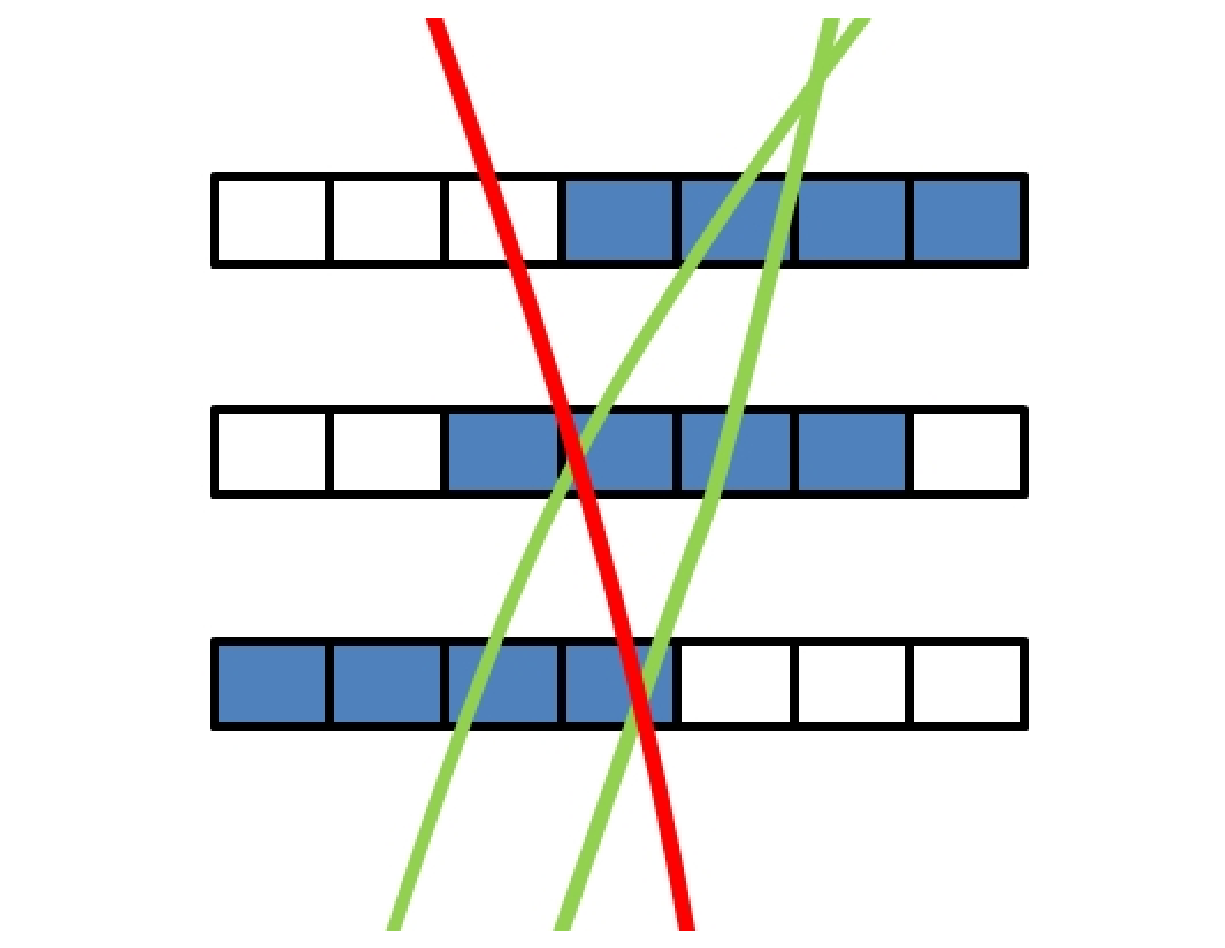
\includegraphics[width=0.3\columnwidth]{Plots/Pattern.eps}
\caption{A pattern in a three-layers detector. Green tracks will match the pattern, red tracks won't.}
\label{fig:pattern}
\end{figure}

\noindent On this picture one also get an idea of the pattern structure. Each pattern is made of one superstrip per layer. A superstrip is a group of strips/pixels, and is therefore heavily constrained by the detector itself. Once the superstrip definition has been set, its position information is coded in a N-bits word: the superstrip address. It is important to realize that the AM-based pattern recognition is using these addresses, and is therefore completely independent from the detector geometry.

\noindent As the addresses are transmitted to the AM independently for each layer, layer number doesn't have to be in the address word. In order to understand the address definition, Fig.~\ref{fig:sstrip_def} shows how a superstrip is defined in the barrel part of the tracker.  
\begin{figure}[ht!]
\centering
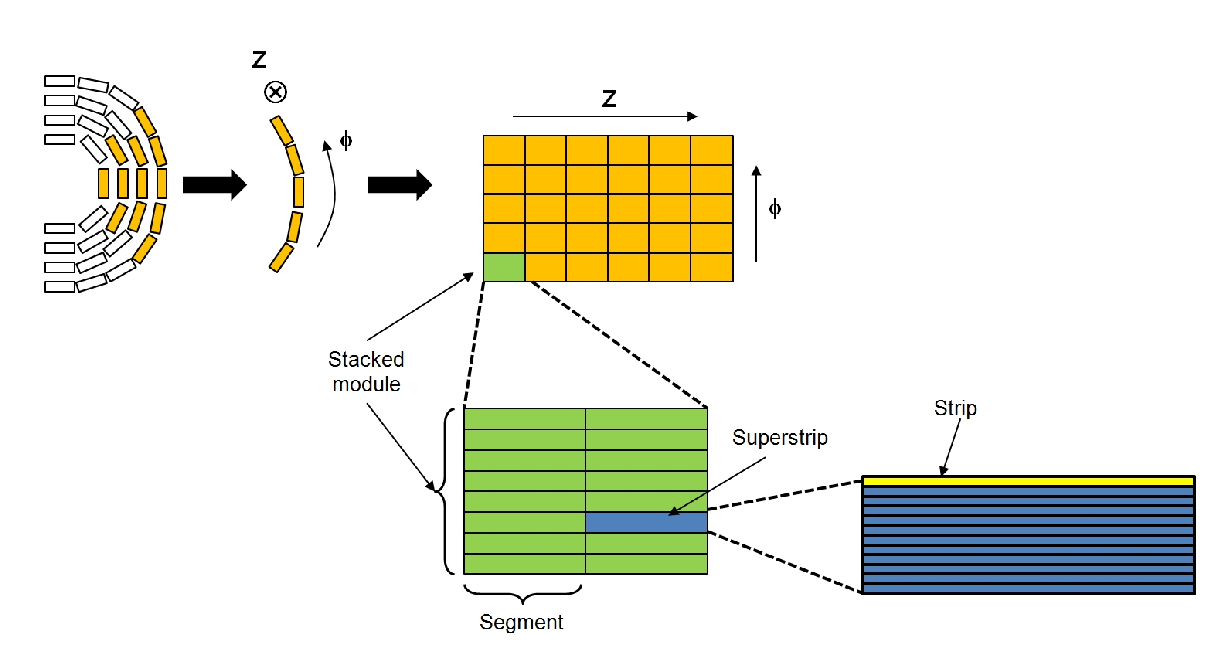
\includegraphics[width=0.7\columnwidth]{Plots/SStripDef.eps}
\caption{Geometric definition of a superstrip (barrel example).}
\label{fig:sstrip_def}
\end{figure}
\begin{figure}[ht!]
\centering
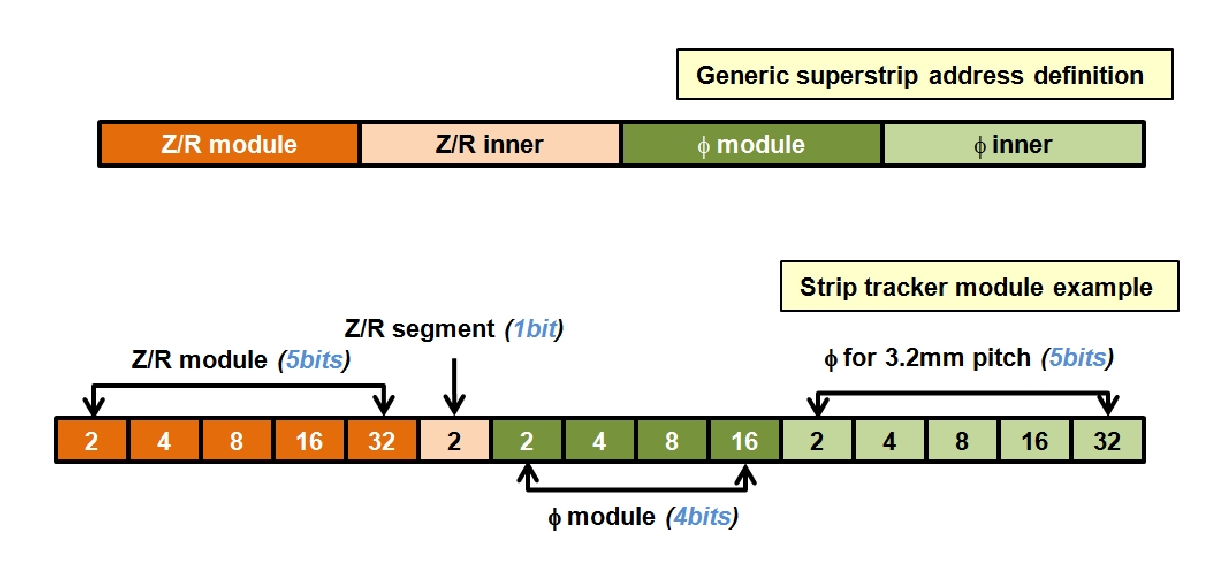
\includegraphics[width=0.7\columnwidth]{Plots/SSaddress.eps}
\caption{Address definition of a superstrip.}
\label{fig:SS_code}
\end{figure}

\noindent One has to be able to define a unique address to define the $z (resp. r)/\phi$ position of each superstrip in the barrel (resp. endcap) sector (r (resp. z) is given by the layer (resp. disk). The coding is sketched on Fig.~\ref{fig:SS_Code}. The number of bits necessary reflects the superstrip granularity and is constrained by the maximal word size acceptable by the AM chip (currently 16 bits). A first set of bits provides the module number along the corresponding coordinate: 5 bits for $Z$ (one could have up to 24 modules in Z in one sector) and 4 for $\phi$ (up to 11 modules per sector in the outermost layer). Then, for each coordinates, a second serie of bits provide the superstrip position within the module. Fig.~\ref{fig:sstrip_def} shows a tracker strip module (in green), divided into 2 segments in $Z$ and 1024 strip in $\phi$. Therefore in order to describe all the position, one would need only 1 bit for $Z$, and 10 bits for $\phi$. In practice, a certain number of strips are grouped to form the superstrip, in our case 32, thus leading to 5 in the address.   

\noindent For the endcap the coding is the same. z is just replaced by r (equivalence is made between disks and layers, ladders and rings). 


\clearpage

\section{Simulation tool development}

\subsection{The importance of simulation tools}

\noindent AM-based L1 tracking is a relatively complex task requiring a precise modelization before going to hardware implementation. This modelization is done via a dedicated simulation framework comprising:

\begin{itemize}
\item The model of the new tracker geometry implemented within the official CMS software chain (CMSSW)
\item The definition of the trigger tower
\item The definition and the production of the pattern banks for each trigger tower
\item The emulation of the AM-based pattern recognition within CMSSW
\item A set of track fitting procedures compatible with an FPGA implementation, coded within CMSSW
\end{itemize}

\noindent The following sections of this part are providing a description of the different steps necessary to setup this modelization. 

\subsection{Tracker geometry and trigger tower definition}

\noindent The geometry description and the trigger sector definition is provided by a standalone program: the TkLayout tool~\cite{bib:TkLayout}. For the geometry, this tool builds the xml files necessary to the CMSSW simulation stage. Then, using rates obtained from simulation and L1 tracking trigger requirements (in particular the minimal $p_T$ required for the tracks), the TkLayout tool can be used to optimize the trigger towers definitions. The goal here is to define the largest possible towers with a reasonable input data rate per layer, and to minimize the data sharing between towers. After performing this task, the TkLayout tool provides a simple text file containing, for each sector, a list of the tracker modules belonging to that sector. This file defines the structure of the track trigger system, and is hence is the basis of the L1 tracking stage.
  
\subsection{Pattern bank generation}

\noindent Bank generation is done via a dedicated standalone C++ program~\cite{bib:AMEmulator}. The main bank generation procedure is sketched on Fig.~\ref{fig:BkGen}. In order to produce a bank, two inputs are needed: a large simulated sample of single particle gun events (traditionally muons) covering the whole L1 track trigger acceptance requirements, and the TkLayout file providing the trigger towers definition.

\begin{figure}[ht!]
\centering
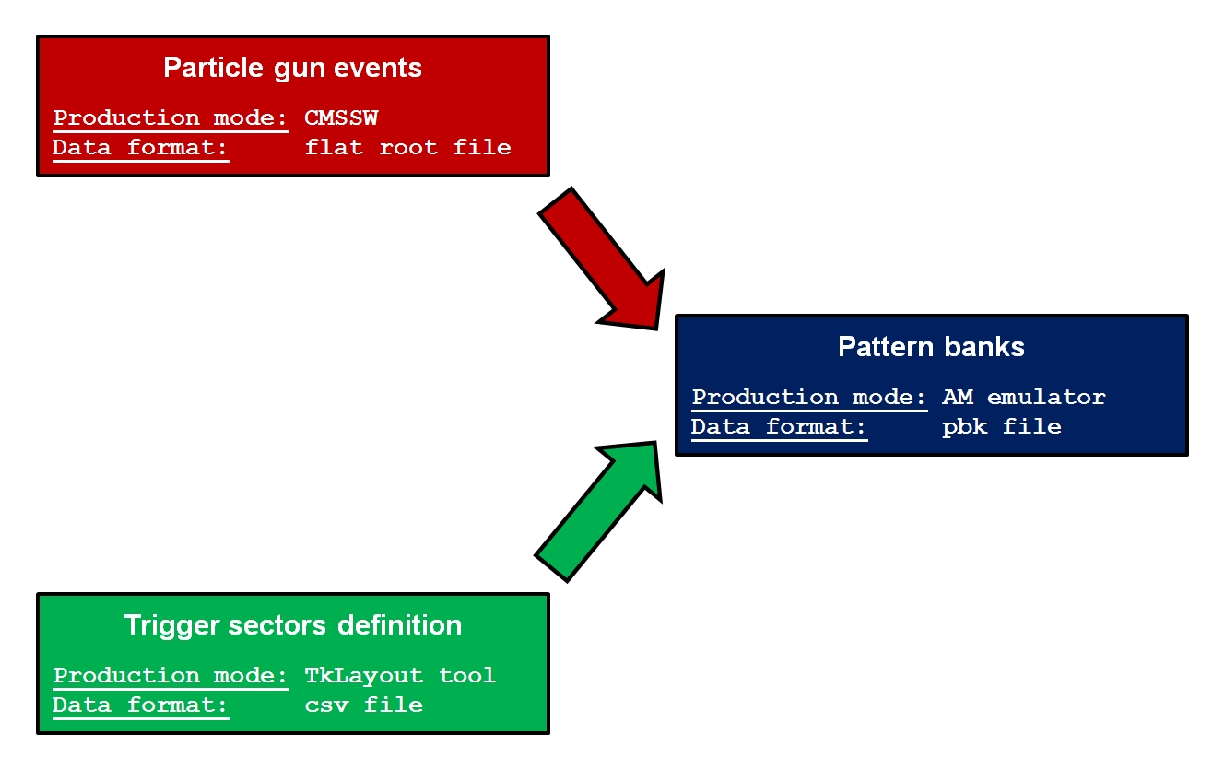
\includegraphics[width=0.6\columnwidth]{Plots/BankGen.eps}
\caption{Pattern bank generation principle}
\label{fig:BkGen}
\end{figure}

\noindent Based on these inputs, the code is able to produce a pattern bank for any trigger tower. Bank parameters can be set in the configuration file of the generation job. A complete description of the available option is provided in~\cite{bib:AMEmulator}.  

\noindent The bank generation algorithm, as it is implemented in the emulator, is summarized on Fig.~\ref{fig:BkGenDet}.

\begin{figure}[ht!]
\centering
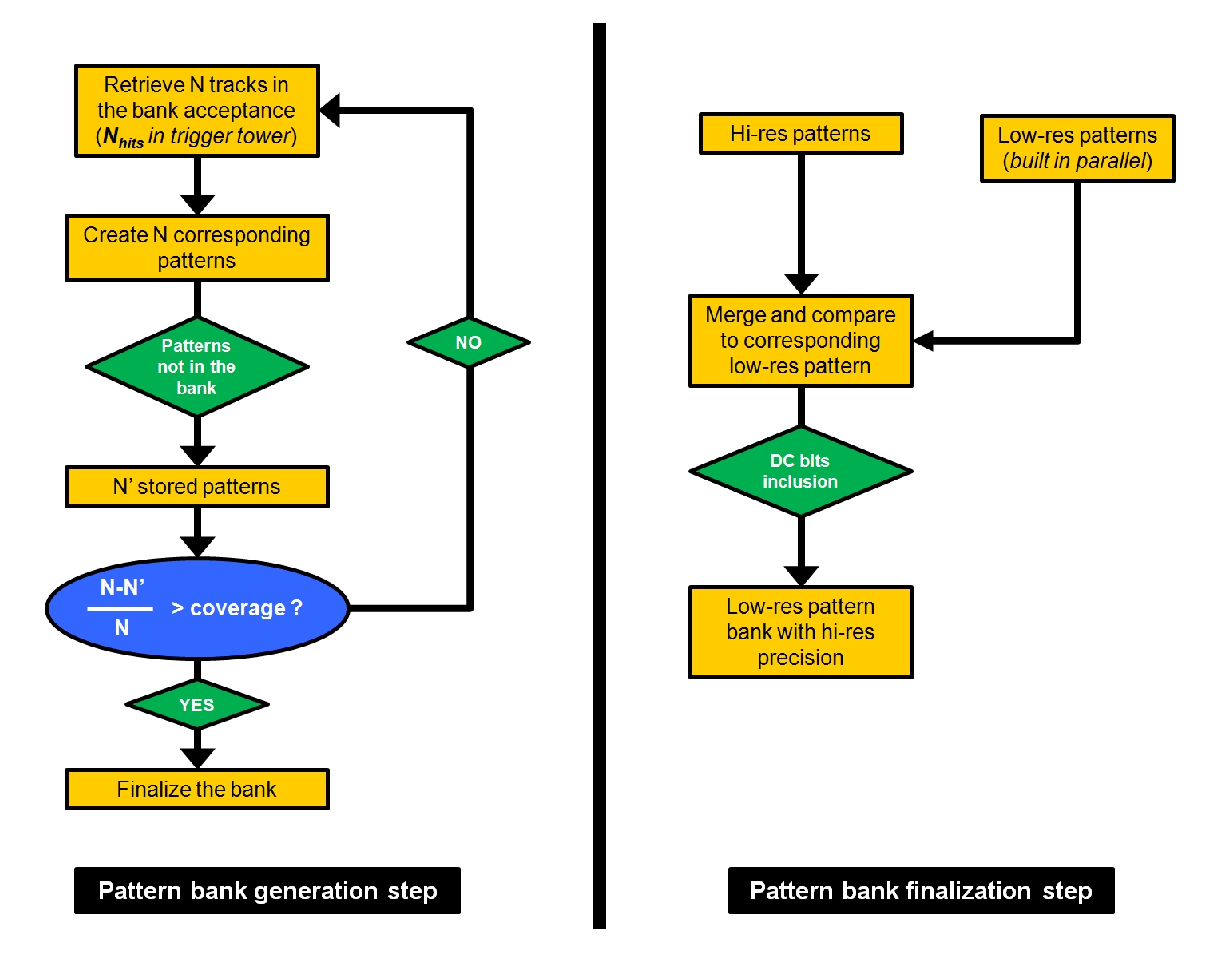
\includegraphics[width=0.6\columnwidth]{Plots/BankGenDetail.eps}
\caption{Pattern bank generation workflow: from track sample to pattern bank}
\label{fig:BkGenDet}
\end{figure}

\noindent This algorithm can be divided into two steps: bank production and bank finalization. As shown on the left diagram, the bank production is performed iteratively. An iteration starts by the collection of a set of $N$ tracks satisfying the pattern bank acceptance requirements in the input data sample (in our case $N=40000$). This acceptance requirement is defined by the parameter $N_{hits}$, which corresponds to the number of different layer/disks in which the particle has induced stubs in the trigger tower considered\footnote{This number should not be confused with the total number of stubs induced by the particle. If a track induces two stubs in a given layer (for example in an overlap area), these stubs will just count as one in $N_{hits}$.}.

\noindent A track can be used to produce a pattern only if its $N_{hits}$ value is equal to the pattern size set in the job configuration. Of course the pattern made from the track is stored in the bank only if not already in. Iteration ends when $N$ tracks have been collected. At this point, the proportion of tracks collected which were leading to an already stored pattern is computed. If this proportion, defined as the bank coverage, is larger than the coverage initially required, the iteration stage stops.

\noindent Once the required coverage has been reached, the bank is finalized. The procedure is described in the right part of Fig.~\ref{fig:BkGenDet}. At this point, it's not one, but two banks which have been built. Indeed, each new pattern is automatically linked to a low-resolution mother pattern. The resolution of this mother pattern is direclty related to the number of DC bits. The width of the low-res patterns is indeed $2^{N_{DC}}$ larger than the width of the high-res ones. For example, if one requires 2 DC bits, and built pattern with a superstrip size of 32 strips, the width of the low resolution patterns will be 128 strips. 

\noindent The low-res bank building follows the same procedure than the hi-res bank. But in addition, each low-res patterns is linked to a set of hi-res patterns. Before storing the low-res pattern in the banks, hi-res patterns belonging to it are merged. The merging result is then compared to the low-res pattern, and the hi-res granularity is kept whenever possible. On the other hand, if all the super-strips are used in a given layer, corresponding DC bits are applied.

\noindent Using this procedure provides the possibility to get high-resolution precision for the price of a low resolution bank. 


\subsection{Pattern recognition}

\subsubsection{Software principle}

\noindent The pattern recognition is done using the same code than the bank generation. This code has been interfaced with the CMS software framework (CMSSW). It uses the official CMSSW stubs and stores the patterns as official CMSSW track seeds. For debugging purposes, the pattern recognition code can also work standalone, starting from plain rootuple containing the stubs of a given event. 

\noindent The code is working for a given sector. The complete pattern recognition of a given event therefore requires to run in parallel jobs for every trigger tower. The data merging is performed afterwards, so that the final output contains for each event the pattern recognition outcome for all the towers. 


\subsubsection{Estimation of the pattern recognition efficiencies and fake rates}

\noindent The basis of the pattern recognitionefficiency is the number $N$ of matchable tracks. This number is depending on the size of the patterns stored. For patterns made of 6 superstrips, if a missing hit is accepted, any track crossing at least 5 layers in the tower will matchable. 

\noindent The number of layers/disks crossed by the particle within one tower is therefore an important parameter. From now own, it will be mentioned in all the notations. For example, $N_{5}$ corresponds to the number of tracks crossing at least 5 layers/disks in one of the trigger tower.

\noindent Starting from there, the efficiency for a given threshold could be defined as the number of tracks matched in a pattern divided by the total number of tracks: 
\begin{equation}
\epsilon_i = \frac{N^{matched}_i}{N_i}
\end{equation} 

\noindent Then, we define the fake rate as the proportion of patterns which are not containing a good track. 
\begin{equation}
\rho_i = \frac{N^{bad patterns}_{i}}{N^{patterns}_{i}}
\end{equation} 

\noindent This fake rate definition doesn't account for the duplicated patterns. This value is measured by the redundancy,which corresponds to the average number of patterns activated by each good track. The ideal pattern bank for a given threshold $i$ is the one for which $\epsilon_i = 1$ and $\rho_i = 0$.

\noindent Such a bank exists, this is the one for which each possible track in the detector corresponds to one pattern. However, the size of such bank will be prohibitive. On the other side, one could imagine the simplest bank with 1 single pattern defined by the whole detector. Such a bank will have $\epsilon=1$, $\rho = 0$ and $r = 1$, but $\epsilon_{hits}$ will be close to 0. Such a solution would be highly inefficient, as TF would be impossible to process. Therefore the optimal solution lies in between, and one realizes that a parameter will be very important: the size of the patterns. The patterns will have to be sufficiently small in order to get a reasonable $\epsilon_{hits}$, but also sufficiently large in order get a reasonable pattern bank size. 

\noindent Finding the optimal bank is a complex exercise which will be done for the TDR, and hence is beyond the scope of this preparatory note. In this document we present preliminary results obtained using a simple set of pattern banks, which where produced using a large sample of particle gun $\mu^{\pm}$ produced within the following phase space:
\begin{itemize}
\item $0 < \eta_0 < 2.2$.
\item $1.95GeV/c < p_{T_0} < 100GeV/c$, generated randomly in $1/p_T$.
\item $-15cm < z_0 < 15cm$.
 \item $-1mm < d_0 < 1mm$.
\end{itemize}  

\noindent In order to cover correctly the whole $pT$ phase space the sample was divided into three $pT$ ranges: 1.95 to 5 GeV/c, 5 to 20, and 20 to 100. Patterns were made from 32 to 256 strips-wide superstrips (we generate 32 strips banks and used 3 DC bits) in order to get banks of ~1M patterns for each trigger tower. The total number of patterns necessary to cover all the tracker in this configuration is 64~Millions. 

\noindent The following table summarizes the overall efficiencies and fake rates obtained for simple single particles with $p_T>2GeV/c$ using the banks described previously, for $N_{hits}=5$.

\begin{table}[ht!]
\centering
\begin{tabular}{|c|c|c|c|}
  \hline
  Particle type & Muons & Pions & Electrons \\ \hline
  Efficiency ($\epsilon_5$, in \%) &  &  &  \\ \hline
  Fake rate ($\rho_5$, in \%) &  &  &  \\\hline
\end{tabular}
\caption{Stub repartition in the tracker, measured with PU=200 events.}
\label{tad:dev}
\end{table}

\noindent Figures~\ref{fig:PRMU} and {fig:PRELE} shows a summary of the pattern recognition outcome for muons and electrons respectively. The broader turn-on for electrons is mainly due to multiple scattering.

\begin{figure}[ht!]
\begin{minipage}[t]{7.5cm}
\centering
%\includegraphics[width=0.75\textwidth]{Plots/Muon.eps}
\caption{Pattern recognition efficiency for single muons}
\label{fig:PRMU}
\end{minipage}
\hfill
\begin{minipage}[t]{7.5cm}
\centering
%\includegraphics[width=0.75\textwidth]{Plots/AdapSec.eps}
\caption{Pattern recognition efficiency for single electrons}
\label{fig:PRELE}
\end{minipage}
\end{figure} 

\noindent In order to evaluate the fake rate, two types of events were used. Both were overlaid with an average of 140 minimum bias events. In the first set, a single muon was added to minbias contents, whereas in the other sample, a four tops final state was added. This last sample could be considered as a worst case scenario for tracker occupancy, and is therefore particularly useful for studying the maximum rates per modules.   

\noindent The pattern recognition efficiency was also tested, as shown on Fig.~\ref{fig:PR_4tops} for the 4 tops events. As expected, the efficiency is robust against pileup. If a pattern is matched, it will always match independently from the stubs you add around it. What will change is the fake proportion. The fake rates, for both samples are summarized in the following table:

\begin{table}[ht!]
\centering
\begin{tabular}{|c|c|c|c|}
  \hline
  Particle type & Muons & Pions & Electrons \\ \hline
  Efficiency ($\epsilon_5$, in \%) &  &  &  \\ \hline
  Fake rate ($\rho_5$, in \%) &  &  &  \\\hline
\end{tabular}
\caption{}
\label{tad:dev}
\end{table}

\subsubsection{Bank efficiency definition}


\subsection{Further developments and improvements}


\clearpage

\section{Track Trigger Performance Requirements}

\subsection{Tracking performance}

\subsection{Performance on trigger objects}

\subsection{Selected physics cases}

\clearpage

\section{Vertical Slice Demonstrator System}

\subsection{System overview}



\clearpage

\section{Project organization}

\subsection{Institutions involved}

\subsection{Schedule and integration plan}

\subsection{Cost estimate}

\clearpage

\input{08_Conclusion}


%----------------------------------------
% Pour la bibliographie
%----------------------------------------

\newpage
\thispagestyle{empty}

\begin{thebibliography}{99}

%\bibitem{bib:Abb-11} D.~Abbaneo {\it for the CMS collaboration} - {\it "Upgrade of the CMS Tracker with tracking trigger"} - CMS CR -2011/284 (2011)

\bibitem{bib:Rist-89} M. Dell Orso, L. Ristori - {\it "VLSI Structure For Track Finding"} - Nucl.Instr. and Meth. A278 (1989), 436

\bibitem{bib:Ade-06} J. Adelman {\it et al.} - {\it "Real time secondary vertexting at CDF"} - Nucl.Instr. and Meth. A569 (2006), 111

\bibitem{bib:Ade-07} J. Adelman {\it et al.} - {\it "The Silicon Vertex Trigger upgrade at CDF"} - Nucl.Instr. and Meth. A572 (2007), 361

\bibitem{bib:Koh-87} T. Kohonen - {\it "Content-Addressable Memories"} - 2nd edition, New York, Springer- Verlag (1987)

\bibitem{bib:Pag-06} K. Pagiamtzis, A. Sheikholeslami - {\it "Content-Addressable Memory (CAM) Circuits and Archtectures: A Tutorial and Survey"} - IEEE Journal of Solid-State Circuits, Vol. 41, No. 3 (2006), 712


%\bibitem{bib:XML_wiki}\url{https://twiki.cern.ch/twiki/bin/view/CMSPublic/SWGuideGeomDevelopersGuide}

%\bibitem{bib:XML_oscar}\url{https://twiki.cern.ch/twiki/bin/view/CMSPublic/SWGuideOscarProducer}

%\bibitem{bib:G4SHits_cfi}\url{http://cmssw.cvs.cern.ch/cgi-bin/cmssw.cgi/CMSSW/SimG4Core/Application/python/g4SimHits_cfi.py?view=markup}

\bibitem{bib:Ann-06} A. Annovi {\it et al.} - {\it "A VLSI Processor for Fast Track Finding Based on Content Addressable Memories"} - IEEE Transactions on Nuclear Science, vol. 53, no. 4 (2006), 1

\bibitem{bib:Ann-09} A. Annovi {\it et al.} - {\it "The GigaFitter: A next generation track fitter to enhance online tracking performances at CDF"} - Nuclear Science Symposium Conference Record (NSS/MIC), 2009 IEEE (2009), 1143

\bibitem{bib:VIP-11}  - {\it "A New Concept of Vertically Integrated Pattern Recognition Associative Memory (VIPRAM)"} - FERMILAB-CONF-11-709-E, Proceedings of TIPP 2011 conference, Volume 37, 2012, Pages 1973

\bibitem{bib:VIP-12}  - {\it "Development of 3D Vertically Integrated Pattern Recognition Associative Memory (VIPRAM)"} - FERMILAB-TM-2493-CMS-E-PPD-TD

\bibitem{bib:FTK-10}  - {\it "FTK: A Hardware Track Finder for the ATLAS Trigger"} - Technical Proposal (2010)

%\bibitem{bib:Kar-91} V.~Karimaki - {\it "Effective circle fitting for particle trajectories"} - Nucl.Instr. and Meth. A305 (1991), 187

\end{thebibliography}
%----------------------------------------
% Annexes
%----------------------------------------

%\appendix


\end{document}
